\documentclass[11pt]{article}

\usepackage[spanish]{babel}
\usepackage[margin=1in]{geometry}
\usepackage{amsmath, amssymb, amsfonts}
\usepackage{graphicx}
\usepackage{float}
\usepackage{booktabs}
\usepackage{longtable}
\usepackage{array}
\usepackage{calc}
\usepackage{etoolbox}
\usepackage{enumitem}
\usepackage{tcolorbox}
\usepackage{hyperref}
\usepackage{xcolor}
\usepackage{parskip}
\usepackage{csquotes}
\usepackage[backend=biber,style=numeric,sorting=none]{biblatex}
\addbibresource{referencias.bib}

\renewcommand{\_}{\textunderscore\allowbreak{}}
\providecommand{\tightlist}{\setlength{\itemsep}{0pt}\setlength{\parskip}{0pt}}
\setlist{itemsep=2pt, topsep=4pt}
\setlength{\LTpre}{4pt}\setlength{\LTpost}{4pt}

\title{\textbf{Laboratorio 10: Respuestas} \vspace{1em}\\
  Deep Learning y Sistemas Inteligentes - CC3092}
\author{José Antonio Mérida Castejón}
\date{\today}

\begin{document}
\decimalpoint

\maketitle

\begin{tcolorbox}[colback=gray!8, colframe=gray!50, boxrule=0.5pt]
\textbf{Nota:} este informe fue generado con IA (Claude Code) a partir del notebook \texttt{Lab10\_XAI.ipynb}, transcribiendo sus respuestas, tablas y figuras. El detalle del uso de IA está en \texttt{AI.md}.
\end{tcolorbox}

El código, las salidas y las gráficas de todos los tasks están en el notebook \texttt{Lab10\_XAI.ipynb}; este documento contiene el enunciado resumido y las respuestas a cada task. Semilla fija: \texttt{SEED = 42}. Las técnicas siguen a Grad-CAM \cite{selvaraju2017} y CAM \cite{zhou2016} en visión, y a SHAP \cite{lundberg2017}, LIME \cite{ribeiro2016} y explicaciones contrafactuales \cite{wachter2017} en datos tabulares.
\section*{Task 1 --- Grad-CAM y CAM sobre ResNet-18}

\subsection*{Task 1.1 --- Modelo, preprocesamiento e imágenes}
\textbf{Instrucciones.}
\begin{itemize}
  \item Cargar ResNet-18 con pesos de ImageNet (\texttt{torchvision}) en modo de evaluación.
  \item Preprocesar: redimensionar a 256 px en el lado corto, recorte central de $224\times224$ y normalización por canal con media $(0.485, 0.456, 0.406)$ y desviación estándar $(0.229, 0.224, 0.225)$.
  \item Elegir tres imágenes (indicando la fuente): (a) un objeto claro y centrado de una clase de ImageNet; (b) dos objetos de clases distintas; (c) un objeto sobre un fondo que pueda engañar al modelo.
  \item Reportar las cinco clases de mayor probabilidad de cada imagen y, para (c), el recuadro del objeto en la imagen de $224\times224$.
\end{itemize}

\begin{figure}[H]
\centering
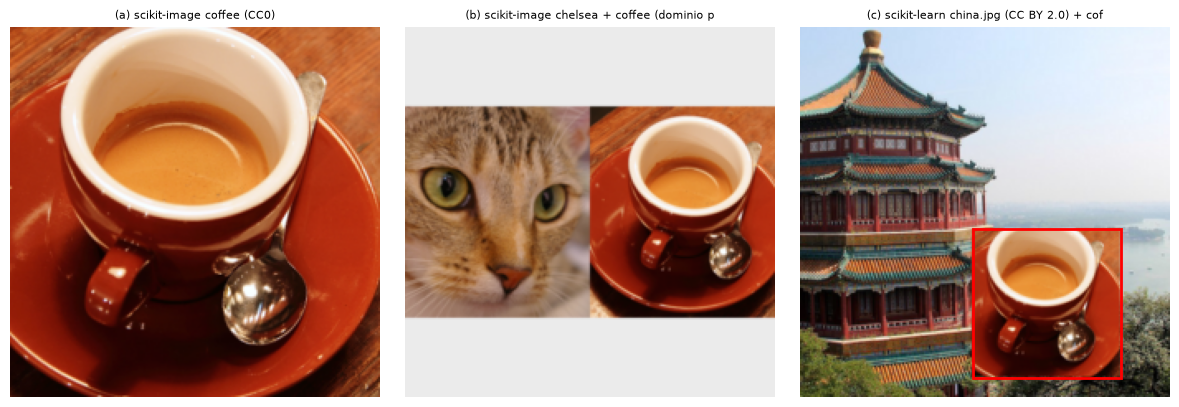
\includegraphics[width=0.9\textwidth]{figs/imagenes.png}
\caption{Las tres imágenes tras el preprocesamiento; el recuadro rojo en (c) encierra la taza pegada sobre el paisaje.}
\end{figure}

\begin{table}[H]
\centering
\small
\begin{tabular}{ll}
\toprule
Imagen & Fuente \\
\midrule
(a) & \texttt{scikit-image} \texttt{coffee} (CC0) \\
(b) & \texttt{scikit-image} \texttt{chelsea} + \texttt{coffee} (dominio público), composición propia \\
(c) & \texttt{scikit-learn} \texttt{china.jpg} (CC BY 2.0) + \texttt{coffee}, composición propia \\
\bottomrule
\end{tabular}
\caption{Fuente de cada imagen.}
\end{table}

\begin{table}[H]
\centering
\small
\begin{tabular}{llll}
\toprule
\# & Imagen (a) & Imagen (b) & Imagen (c) \\
\midrule
1 & espresso (0.852) & cup (0.176) & bell cote (0.274) \\
2 & chocolate sauce (0.040) & Egyptian cat (0.092) & palace (0.204) \\
3 & consomme (0.039) & tabby (0.091) & dome (0.051) \\
4 & soup bowl (0.025) & espresso (0.087) & stupa (0.048) \\
5 & cup (0.020) & loupe (0.039) & boathouse (0.047) \\
\bottomrule
\end{tabular}
\caption{Cinco clases de mayor probabilidad por imagen.}
\end{table}

En (a) el modelo acierta con seguridad (\emph{espresso}, \(\approx\) 0.85). En (b) reparte la probabilidad entre los dos objetos (\emph{cup} \(\approx\) 0.18, gatos \(\approx\) 0.09 cada uno), y en (c) predice la escena (\emph{bell cote} \(\approx\) 0.27, \emph{palace} \(\approx\) 0.20) en lugar de la taza. El recuadro de la taza en (c) es \((104, 122, 194, 212)\) en la imagen de \(224\times224\).


\subsection*{Task 1.2 --- Grad-CAM desde cero}
\textbf{Instrucciones.}
\begin{itemize}
  \item Implementar Grad-CAM sobre \texttt{layer4}: hook de avance para las activaciones $A$ ($512\times7\times7$) y hook de retroceso para $\partial y^c/\partial A$.
  \item Retropropagar desde el logit $y^c$ (antes del softmax), calcular $\alpha_k^c$ como el promedio espacial del gradiente y formar $L^c=\mathrm{ReLU}\big(\sum_k\alpha_k^cA^k\big)$, ampliado a $224\times224$ (bilineal) y normalizado min--max.
  \item Generar el mapa de la clase top-1 de cada imagen y, para (b), también el de la clase del segundo objeto.
\end{itemize}

\begin{figure}[H]
\centering
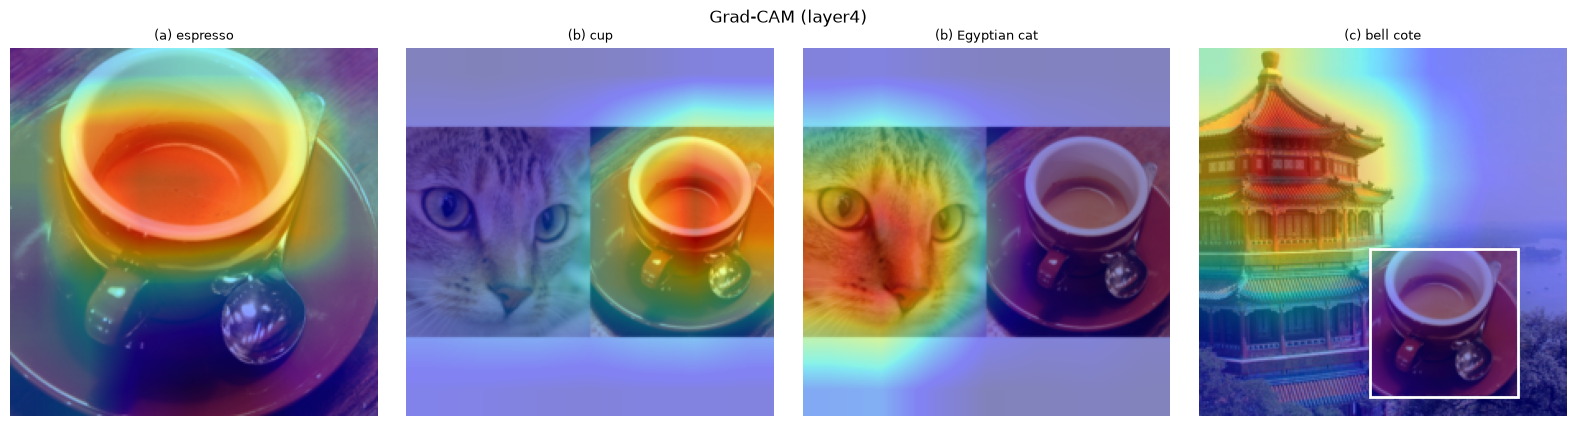
\includegraphics[width=\linewidth]{figs/gradcam.png}
\caption{Grad-CAM (\texttt{layer4}) para la clase top-1 de (a), (b), (c) y la clase del segundo objeto de (b).}
\end{figure}

En (a) el mapa cubre la taza; en (b) cada clase ilumina su propio objeto (taza a la derecha, gato a la izquierda); en (c) el mapa se concentra en el templo y casi no toca la taza dentro del recuadro.


\subsection*{Task 1.3 --- CAM desde los pesos de \texttt{fc}}
\textbf{Instrucciones.}
\begin{itemize}
  \item Calcular $M^c_{ij}=\sum_kw_k^cA^k_{ij}$ con los pesos de \texttt{fc}, sin gradientes.
  \item Verificar la descomposición $\frac1Z\sum_{i,j}M^c_{ij}+b_c=y^c$ ($Z=49$) y reportar ambos valores y el error absoluto.
  \item Comparar $Z\cdot L^c$ (sin ReLU ni normalización) con $M^c$: error absoluto máximo sobre las 49 posiciones.
  \item Aplicar ReLU y normalización min--max a ambos mapas y reportar el error absoluto máximo.
\end{itemize}

\begin{table}[H]
\centering
\small
\begin{tabular}{llrrrrr}
\toprule
Imagen & Clase & $y^c$ & $\frac1Z\sum M+b$ & $|\text{error}|$ (b) & $\max|ZL-M|$ (c) & $\max|\text{norm}|$ (d) \\
\midrule
a & espresso & 15.6166 & 15.6166 & $9.5\times10^{-7}$ & $1.3\times10^{-5}$ & $5.4\times10^{-7}$ \\
b & cup & 9.1934 & 9.1934 & $0$ & $1.1\times10^{-5}$ & $4.2\times10^{-7}$ \\
b (2.º) & Egyptian cat & 8.5515 & 8.5515 & $9.5\times10^{-7}$ & $1.3\times10^{-5}$ & $5.4\times10^{-7}$ \\
c & bell cote & 9.4988 & 9.4988 & $9.5\times10^{-7}$ & $7.6\times10^{-6}$ & $4.8\times10^{-7}$ \\
\bottomrule
\end{tabular}
\caption{Verificaciones de CAM (a)--(d) del Task 1.3.}
\end{table}

En las cuatro comprobaciones los errores son de \(\lesssim10^{-5}\) (precisión de float32): la descomposición del logit se cumple, \(Z\,L^c = M^c\) y los mapas normalizados coinciden. Es decir, en este ResNet Grad-CAM y CAM son el mismo mapa salvo la constante \(Z\).


\subsection*{Task 1.4 --- Preguntas}
\subsubsection*{(a) $\alpha_k^c$ vs.\ $w_k^c/Z$ en la imagen (a)}
\begin{table}[H]
\centering
\small
\begin{tabular}{rrrrr}
\toprule
Canal $k$ & $w_k^c$ & $\alpha_k^c$ & $w_k^c/Z$ & Error relativo \\
\midrule
103 & 0.3137 & 0.0064 & 0.0064 & $0$ \\
432 & 0.2924 & 0.0060 & 0.0060 & $0$ \\
172 & 0.2901 & 0.0059 & 0.0059 & $7.9\times10^{-8}$ \\
14 & 0.2892 & 0.0059 & 0.0059 & $7.9\times10^{-8}$ \\
144 & 0.2474 & 0.0050 & 0.0050 & $9.2\times10^{-8}$ \\
\bottomrule
\end{tabular}
\caption{Cinco canales de mayor peso para la clase de la imagen (a). Error relativo máximo sobre los 512 canales: $2.4\times10^{-7}$ (épsilon de float32: $1.2\times10^{-7}$).}
\end{table}

\begin{tcolorbox}[colback=yellow!12, colframe=orange!70!black, boxrule=0.5pt, left=4pt, right=4pt]
\textbf{Pregunta.} Compare \(\alpha_k^c\) con \(w_k^c/Z\) en los 5 canales de mayor peso (imagen a) y reporte el error relativo. ¿En qué paso de la derivación se usa que \(\partial y^c/\partial A^k_{ij}\) es igual en todas las posiciones? ¿Por qué el error es del orden de la precisión de punto flotante y no cero?
\end{tcolorbox}

Se calculó \(\alpha_k^c\) para la clase de la imagen (a) y se comparó con \(w_k^c/Z\), donde \(Z = 49\) es el número de posiciones espaciales. En los cinco canales de mayor peso, los dos valores son prácticamente iguales. Por ejemplo, en el canal 103 ambos dan aproximadamente \(0.0064\). El error relativo en estos canales es menor a \(10^{-7}\). Al revisar los 512 canales, el error máximo es de alrededor de \(2\times10^{-7}\). Además, el gradiente es idéntico en todas las posiciones de un mismo canal.

Esto se explica por el \emph{global average pooling} antes de la capa final. La salida de la clase es

\[y^c=\sum_k w_k^c\,\frac{1}{Z}\sum_{i,j}A^k_{ij}+b_c,\]

así que al derivar respecto a una activación se obtiene

\[\frac{\partial y^c}{\partial A^k_{ij}}=\frac{w_k^c}{Z}.\]

La derivada no depende de la posición \((i,j)\). Como el gradiente es constante dentro del canal, promediarlo no cambia nada, y entonces \(\alpha_k^c = w_k^c/Z\). Es decir, en esta arquitectura Grad-CAM y CAM dan el mismo mapa, solo escalado por la constante \(Z\).

Los errores no son exactamente cero porque PyTorch trabaja en float32, cuya precisión es de aproximadamente \(1.2\times10^{-7}\). Al calcular el gradiente, PyTorch divide entre 49, multiplica por los pesos y luego promedia, en un orden distinto al del cálculo directo de \(w_k^c/Z\). Cada una de esas operaciones redondea un poco. Por eso los errores son del mismo orden que la precisión de float32.

\subsubsection*{(b) Discriminación entre las dos clases de la imagen (b)}
\begin{figure}[H]
\centering
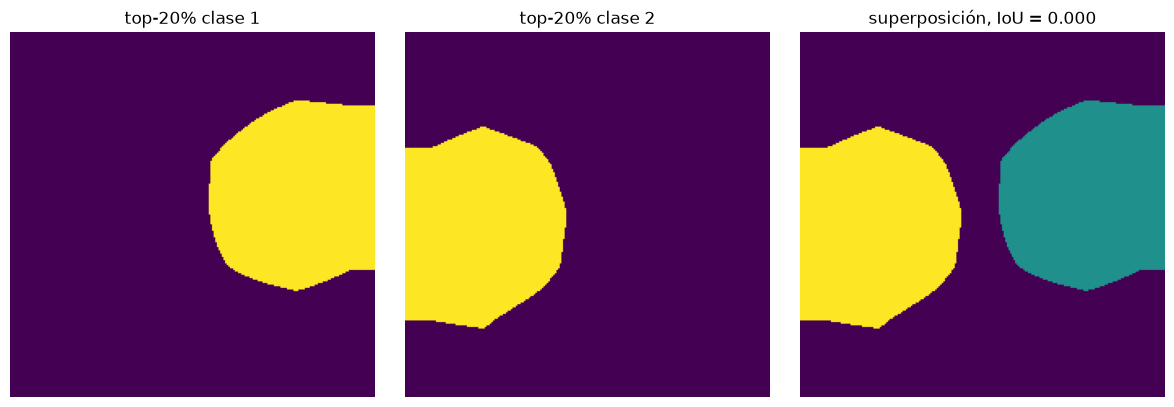
\includegraphics[width=0.85\textwidth]{figs/iou.png}
\caption{Regiones top-20\,\% de cada clase en (b) y su superposición (IoU $=0$).}
\end{figure}

\begin{tcolorbox}[colback=yellow!12, colframe=orange!70!black, boxrule=0.5pt, left=4pt, right=4pt]
\textbf{Pregunta.} En la imagen (b), reporte el IoU entre el 20 \% de píxeles más altos de los mapas de las dos clases. ¿El mapa discrimina entre clases? ¿Qué límite impone que cada posición cubra \(32\times32\) px?
\end{tcolorbox}

El IoU entre las regiones top-20 \% de \emph{cup} y \emph{Egyptian cat} es \(0\). Es decir, las dos regiones no se tocan. Los centros de masa de cada mapa están en lados opuestos de la imagen: la taza en \(x\approx143\) y el gato en \(x\approx58\). Esto coincide con la posición real de cada objeto. Además, la correlación de Spearman entre los dos mapas de \(7\times7\) es \(-0.16\), así que tampoco hay una relación positiva entre ellos.

Por lo tanto, el mapa sí discrimina entre clases; cada clase resalta su propio objeto y no la misma zona. Vale la pena notar que las probabilidades del modelo son bajas (\(\approx\) \(0.18\) para la taza y \(\approx\) \(0.09\) para el gato). Aun así, los mapas son claros, lo que muestra que Grad-CAM puede localizar bien aunque el modelo no esté muy seguro de su predicción.

Que cada posición cubra \(32\times32\) px significa que el mapa no puede localizar nada con más precisión que un bloque de 32 px. Un objeto más pequeño que eso, o dos objetos a menos de 32 px de distancia, quedan dentro de la misma celda y el mapa no los puede separar. Escalar el mapa a \(224\times224\) no lo arregla, porque la interpolación solo suaviza los bordes entre celdas y no agrega información.

\subsubsection*{(c) Imagen (c): masa dentro del recuadro y prueba causal}
\begin{figure}[H]
\centering
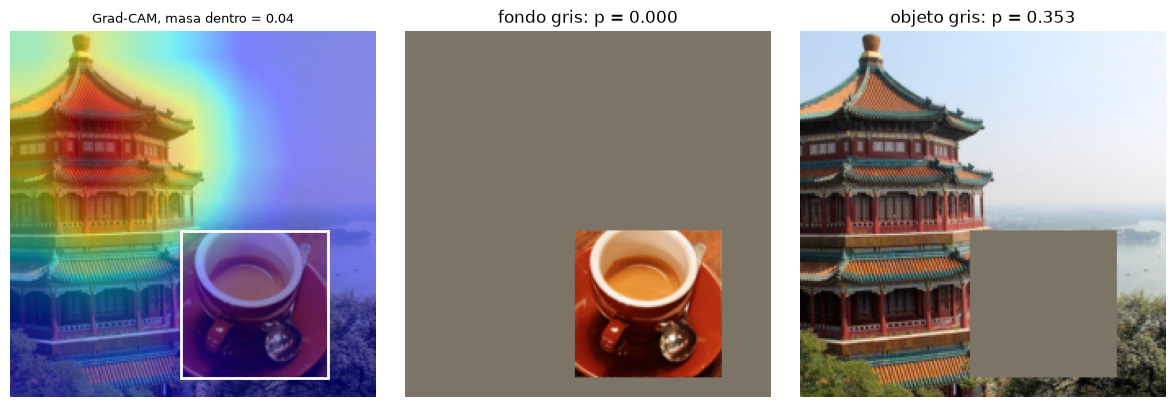
\includegraphics[width=0.9\textwidth]{figs/causal.png}
\caption{Grad-CAM de (c) (masa dentro del recuadro $\approx4$\,\%) y prueba causal con el fondo o el objeto en gris.}
\end{figure}

\begin{tcolorbox}[colback=yellow!12, colframe=orange!70!black, boxrule=0.5pt, left=4pt, right=4pt]
\textbf{Pregunta.} En la imagen (c), ¿qué fracción de la masa del mapa cae dentro del recuadro? Haga la prueba causal (todo lo de fuera en gris) y diga si mapa y prueba coinciden en que el modelo usa el fondo. ¿Hay evidencia de atajo?
\end{tcolorbox}

Solo el \(\approx\) 4 \% de la masa del mapa cae dentro del recuadro, aunque el recuadro ocupa \(\approx\) 16 \% de la imagen. Es decir, el mapa le da al objeto menos atención de la que le tocaría al azar y se concentra en el fondo (el templo).

En la prueba causal, la probabilidad de \emph{bell cote} es \(0.27\) con la imagen original. Al poner el fondo en gris y dejar solo la taza, cae a \(\approx 0\) y el modelo pasa a predecir \emph{espresso} (\(\approx 0.8\)). Al poner la taza en gris y dejar solo el fondo, sube a \(0.35\).

El mapa y la prueba coinciden, el modelo usa el fondo y no la taza. Quitar la taza no baja la predicción, mientras que quitar el fondo la elimina por completo.

Sí hay evidencia de atajo. El modelo clasifica la escena por su contexto e ignora el objeto. Además, el mapa (que es correlacional) y la intervención (que es causal) llegan a la misma conclusión, lo que la hace más confiable.

\newpage
\section*{Task 2 --- SHAP sobre German Credit}

\subsection*{Task 2.1 --- Datos y modelo}
\textbf{Instrucciones.}
\begin{itemize}
  \item Descargar German Credit (1\,000 solicitudes, 20 variables: 7 numéricas y 13 categóricas) con \texttt{fetch\_openml("credit-g", version=1)}.
  \item Codificar \texttt{good}$=1$, \texttt{bad}$=0$ y las categóricas con un codificador ordinal (códigos arbitrarios, tratados como numéricos).
  \item Partición estratificada 80/20 y gradient boosting de \texttt{scikit-learn} (semilla 42, 200 árboles, profundidad máxima 3, fondo SHAP de 100 instancias).
  \item Reportar exactitud y AUC en el conjunto de prueba.
\end{itemize}

\begin{table}[H]
\centering
\small
\begin{tabular}{lr}
\toprule
Métrica (prueba) & Valor \\
\midrule
Exactitud & 0.775 \\
AUC & 0.765 \\
\bottomrule
\end{tabular}
\caption{Desempeño del modelo en el conjunto de prueba.}
\end{table}

El modelo alcanza una exactitud de \(\approx\) 0.78 y un AUC de \(\approx\) 0.77 en prueba: un desempeño moderado, suficiente para explicarlo pero sin mucho margen. Los códigos ordinales de las categóricas son arbitrarios y el modelo los trata como numéricos, lo cual limita la interpretación de esas variables.


\subsection*{Task 2.2 --- TreeSHAP intervencional}
\textbf{Instrucciones.}
\begin{itemize}
  \item Calcular los valores SHAP del conjunto de prueba (TreeSHAP intervencional, log-odds, fondo de 100 instancias).
  \item (a) Verificar la eficiencia: $\phi_0+\sum_j\phi_j=f(x)$, error absoluto máximo. (b) Verificar que el valor base es el promedio de $f$ sobre el fondo.
  \item (c) Importancia global $I_j=\frac1N\sum_n|\phi_j^{(n)}|$ e importancia por permutación (AUC, 10 repeticiones): cinco variables principales de cada una y correlación de Spearman entre los rankings.
  \item (d) Cliente de prueba con $p>0.8$ y otro con $p<0.2$: cascadas, descripción de sus tres contribuciones más grandes y beeswarm global.
\end{itemize}

\begin{table}[H]
\centering
\small
\begin{tabular}{lr}
\toprule
Verificación & Resultado \\
\midrule
(a) Error máximo de eficiencia & $9.5\times10^{-8}$ \\
(b) Valor base $\phi_0$ & 1.3345 \\
(b) Promedio de $f$ en el fondo & 1.3345 \\
\bottomrule
\end{tabular}
\caption{Eficiencia y valor base.}
\end{table}

\textbf{(a) y (b).} El error absoluto máximo de eficiencia es bastante pequeño (\(\approx10^{-7}\)), además la diferencia entre el valor base y el promedio de la salida en log-odds es prácticamente 0 (ambos \(\approx1.33\)). Todo cuadra.

\begin{table}[H]
\centering
\small
\begin{tabular}{lll}
\toprule
Rank & SHAP $I_j$ & Permutación $\Delta$AUC \\
\midrule
1 & checking\_status (0.735) & checking\_status (0.119) \\
2 & credit\_amount (0.487) & credit\_amount (0.076) \\
3 & purpose (0.484) & duration (0.058) \\
4 & duration (0.378) & credit\_history (0.040) \\
5 & savings\_status (0.340) & savings\_status (0.026) \\
\bottomrule
\end{tabular}
\caption{Cinco variables principales por cada importancia. Spearman entre los rankings completos: $\rho=0.702$.}
\end{table}

\textbf{(c).} El Spearman entre rankings es 0.702, por lo cual ambos rankings están bastante correlacionados. Las cinco variables principales según SHAP son:

\begin{itemize}
\tightlist
\item
  \texttt{checking\_status}
\item
  \texttt{credit\_amount}
\item
  \texttt{purpose}
\item
  \texttt{duration}
\item
  \texttt{savings\_status}
\end{itemize}

Según permutación son:

\begin{itemize}
\tightlist
\item
  \texttt{checking\_status}
\item
  \texttt{credit\_amount}
\item
  \texttt{duration}
\item
  \texttt{credit\_history}
\item
  \texttt{savings\_status}
\end{itemize}

\begin{figure}[H]
\centering
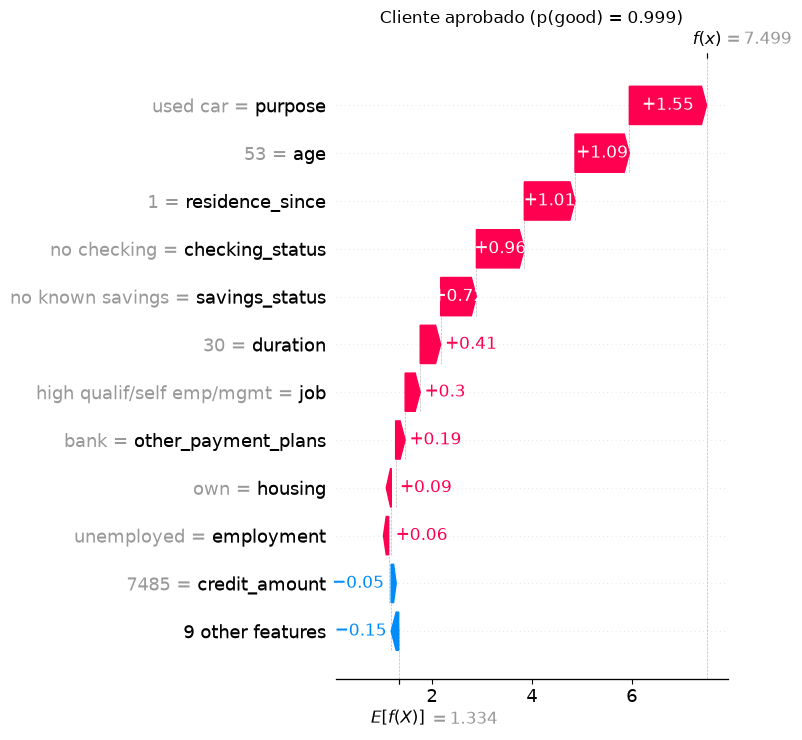
\includegraphics[width=0.62\textwidth]{figs/waterfall_aprobado.png}
\caption{Cascada del cliente aprobado ($p=0.999$).}
\end{figure}

\begin{figure}[H]
\centering
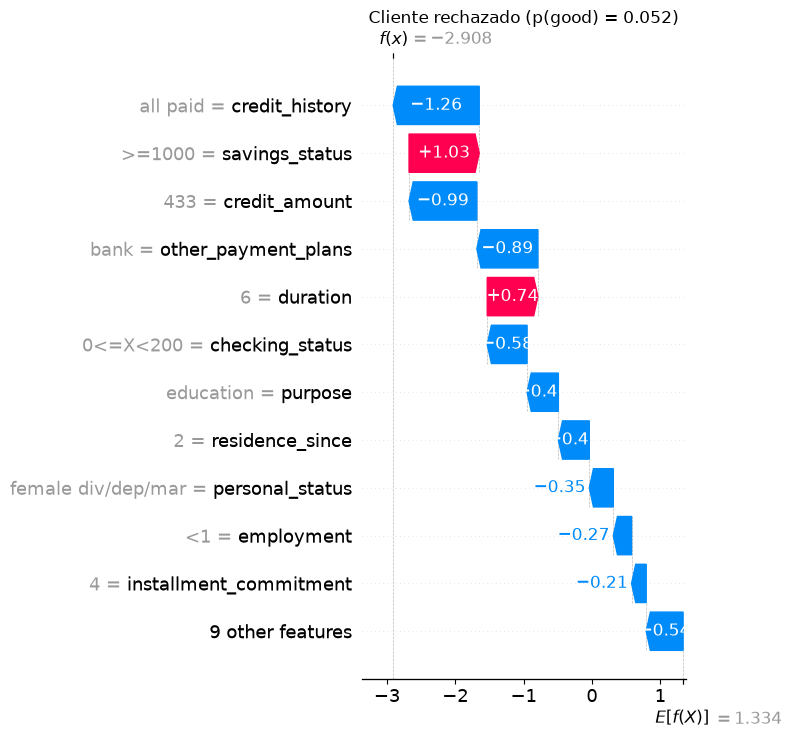
\includegraphics[width=0.62\textwidth]{figs/waterfall_rechazado.png}
\caption{Cascada del cliente rechazado ($p=0.052$).}
\end{figure}

\begin{figure}[H]
\centering
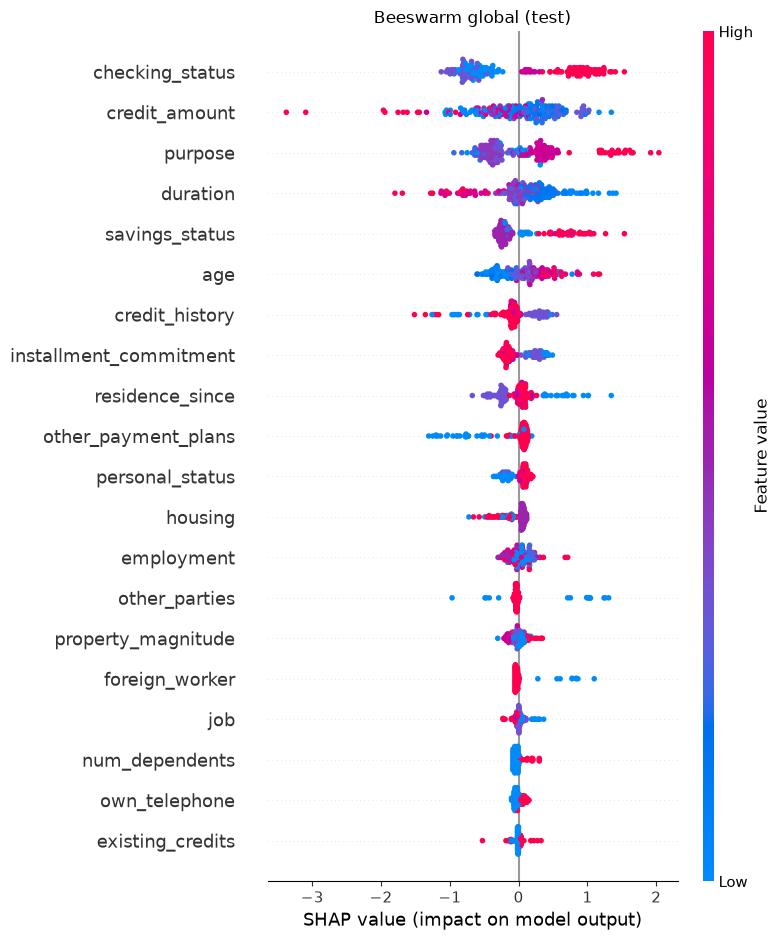
\includegraphics[width=0.62\textwidth]{figs/beeswarm.png}
\caption{Beeswarm global de los valores SHAP en prueba.}
\end{figure}

\textbf{(d).} \begin{tcolorbox}[colback=yellow!12, colframe=orange!70!black, boxrule=0.5pt, left=4pt, right=4pt]
\textbf{Pregunta.} Describa con palabras las tres contribuciones más grandes del cliente aprobado (\(p>0.8\)) y del rechazado (\(p<0.2\)).
\end{tcolorbox}

El valor base es \(\phi_0 = 1.334\) log-odds, que equivale a \(\approx\) 79 \% de probabilidad de \emph{good} para un cliente promedio.

El cliente aprobado (índice 50, \(p = 0.999\)) tiene tres contribuciones grandes, y las tres a favor. Que el préstamo sea para un carro usado suma \(+1.55\), tener 53 años suma \(+1.09\) y llevar 1 año en su residencia actual suma \(+1.01\). Entre las tres aportan más de la mitad de lo que el cliente suma por encima de la base, y llevan la probabilidad casi a 1.

En el cliente rechazado (índice 76, \(p = 0.052\)), la contribución más grande es su historial de crédito ``all paid'', que resta \(-1.26\). Le siguen tener ahorros de 1000 o más, que suma \(+1.03\), y el monto del crédito (433), que resta \(-0.99\). Los ahorros ayudan, pero no alcanzan: varias contribuciones negativas medianas, como \texttt{other\_payment\_plans} (\(-0.89\)) y \texttt{checking\_status} (\(-0.58\)), terminan bajando el log-odds de \(+1.33\) a \(-2.91\).

Llama la atención que tener todo pagado \emph{reduzca} la probabilidad de ser buen cliente. Es contraintuitivo, y refleja un patrón de los datos (y de una codificación ordinal arbitraria), no una regla de negocio razonable.

\subsection*{Task 2.3 --- Variable redundante}
\textbf{Instrucciones.}
\begin{itemize}
  \item Tomar la variable numérica de mayor $I_j$ y crear una copia con ruido $x_{dup}=x+0.05\,\sigma_x\epsilon$, $\epsilon\sim\mathcal N(0,1)$.
  \item Reentrenar con 21 variables (misma semilla) y calcular SHAP con la configuración intervencional (con fondo) y con \texttt{tree\_path\_dependent}.
  \item Presentar una tabla con el promedio de $|\phi|$ de la variable original y de su copia, y el promedio de $|\phi_{orig}+\phi_{copia}|$, y compararla con el $I_j$ del modelo sin copia.
\end{itemize}

\begin{table}[H]
\centering
\small
\begin{tabular}{lrrrr}
\toprule
Configuración & mean$|\phi_{orig}|$ & mean$|\phi_{copia}|$ & mean$|\phi_{orig}+\phi_{copia}|$ & $I_j$ sin copia \\
\midrule
Intervencional (fondo 100) & 0.303 & 0.306 & 0.501 & 0.487 \\
\texttt{tree\_path\_dependent} & 0.275 & 0.293 & 0.481 & 0.487 \\
\bottomrule
\end{tabular}
\caption{Variable duplicada: \texttt{credit\_amount} (correlación original--copia $0.999$).}
\end{table}

El crédito de \texttt{credit\_amount} se reparte casi por igual entre la variable y su copia (\(\approx\) 0.30 cada una en la intervencional y \(\approx\) 0.28--0.29 en la de trayectoria), y la suma \(|\phi_{orig}+\phi_{copia}|\) (\(\approx\) 0.50 y \(\approx\) 0.48) queda cerca del \(I_j\) sin copia (\(\approx\) 0.49). Cada una por separado parece menos importante de lo que es la variable original.


\subsection*{Task 2.4 --- KernelSHAP vs.\ TreeSHAP}
\textbf{Instrucciones.}
\begin{itemize}
  \item Calcular KernelSHAP (log-odds, 2\,000 muestras por instancia) para 10 instancias de prueba con fondos de 10, 50 y 100 instancias.
  \item Para cada fondo, reportar el error absoluto medio respecto a TreeSHAP intervencional con el mismo fondo y el tiempo de cómputo.
\end{itemize}

\begin{table}[H]
\centering
\small
\begin{tabular}{rrrrr}
\toprule
Fondo & MAE vs.\ TreeSHAP & Error máx. & $t$ Kernel (s) & $t$ Tree (s) \\
\midrule
10 & 0.0023 & 0.0159 & 0.257 & 0.0014 \\
50 & 0.0040 & 0.0252 & 0.717 & 0.0058 \\
100 & 0.0038 & 0.0230 & 1.357 & 0.0111 \\
\bottomrule
\end{tabular}
\caption{KernelSHAP frente a TreeSHAP (10 instancias).}
\end{table}

KernelSHAP queda muy cerca de TreeSHAP con los tres fondos (error medio \(\approx\) 0.002--0.004), y no mejora al aumentar el fondo. El tiempo sí crece con el fondo (\(\approx\) 0.25 s con 10, \(\approx\) 0.7 s con 50 y \(\approx\) 1.35 s con 100 instancias) y es mucho mayor que el de TreeSHAP (milisegundos).


\subsection*{Task 2.5 --- Shapley exacto escrito a mano}
\textbf{Instrucciones.}
\begin{itemize}
  \item Entrenar un segundo modelo con seis variables numéricas (\texttt{duration, credit\_amount, installment\_commitment, residence\_since, age, existing\_credits}) y un fondo de 50 instancias.
  \item Para 5 instancias de prueba: definir $v(S)$ como el promedio de la salida (log-odds) sobre el fondo fijando en la instancia las variables de $S$; enumerar las $2^6=64$ coaliciones y calcular cada $\phi_i$ con la fórmula de Shapley (pesos con factoriales).
  \item Comparar con el explicador de árboles intervencional (error máximo) y verificar la eficiencia: $\sum_i\phi_i=v(N)-v(\emptyset)$.
\end{itemize}

\begin{table}[H]
\centering
\small
\begin{tabular}{rrrrr}
\toprule
Instancia & $\max|\phi^{propio}-\phi^{shap}|$ & $\sum\phi$ & $v(N)-v(\emptyset)$ & $|$error eficiencia$|$ \\
\midrule
0 & $3.3\times10^{-9}$ & 0.2521 & 0.2521 & $2.2\times10^{-16}$ \\
1 & $1.0\times10^{-8}$ & $-1.6235$ & $-1.6235$ & $0$ \\
2 & $1.6\times10^{-8}$ & $-0.6183$ & $-0.6183$ & $4.4\times10^{-16}$ \\
3 & $1.1\times10^{-8}$ & 1.4483 & 1.4483 & $2.2\times10^{-16}$ \\
4 & $2.1\times10^{-8}$ & 0.0808 & 0.0808 & $7.4\times10^{-16}$ \\
\bottomrule
\end{tabular}
\caption{Shapley exacto propio frente a TreeSHAP (error máximo global $2.1\times10^{-8}$).}
\end{table}

El cálculo exacto con la fórmula de Shapley coincide con el explicador de árboles (error máximo \(\approx\) \(10^{-8}\)) y los \(\phi_i\) suman \(v(N)-v(\emptyset)\) hasta precisión de máquina, así que la implementación es correcta.


\subsection*{Task 2.6 --- Preguntas}
\subsubsection*{(a) Aditividad en log-odds vs.\ probabilidad (cliente rechazado)}
\begin{tcolorbox}[colback=yellow!12, colframe=orange!70!black, boxrule=0.5pt, left=4pt, right=4pt]
\textbf{Pregunta.} Para el cliente rechazado calcule \(p(x)\), \(\sigma(\phi_0)\) y \(\sum_j[\sigma(\phi_0+\phi_j)-\sigma(\phi_0)]\); compárela con \(p(x)-\sigma(\phi_0)\). ¿Por qué SHAP suma exacto en log-odds pero no en probabilidad?
\end{tcolorbox}

Para el cliente rechazado, \(p(x) \approx 0.05\) y \(\sigma(\phi_0) \approx 0.79\), así que la caída real es \(p(x) - \sigma(\phi_0) \approx -0.74\). La suma de los efectos individuales en probabilidad da \(\approx -0.97\). Es decir, sumar los efectos uno por uno exagera la caída en \(\approx\) \(0.23\).

SHAP suma exacto en log-odds porque esa es la función que explica: \(f(x) = \phi_0 + \sum_j \phi_j\). En este caso el error es de \(\sim10^{-7}\), o sea, cero en la práctica. Pero la probabilidad es \(\sigma(f(x))\), y como la sigmoide no es lineal, el efecto de sumar todo junto no es igual a la suma de los efectos por separado.

La razón concreta es la pendiente de la sigmoide. Cada efecto individual se mide partiendo de \(\phi_0\), donde la sigmoide es empinada, así que cada uno parece mover mucho la probabilidad. Pero cuando las contribuciones negativas se acumulan, el cliente llega a la cola de la sigmoide, donde la curva es plana y cada contribución adicional mueve muy poco la probabilidad. Por eso la suma individual sobreestima la caída real.

\subsubsection*{(b) Mayor discrepancia de ranking SHAP vs.\ permutación}
\begin{tcolorbox}[colback=yellow!12, colframe=orange!70!black, boxrule=0.5pt, left=4pt, right=4pt]
\textbf{Pregunta.} ¿Qué variable tiene la mayor diferencia de posición entre el ranking de \(I_j\) y el de permutación? Proponga una hipótesis respaldada por datos y explique qué mide cada importancia.
\end{tcolorbox}

La variable con mayor diferencia es \texttt{age}. Está en el puesto 6 según SHAP (\(I_j = 0.292\)), pero en el puesto 20 según permutación, donde su efecto (\(\Delta\text{AUC} = -0.005 \pm 0.010\)) no se distingue de cero.

La hipótesis es que el modelo sobreajusta con \texttt{age}: la usa mucho, pero lo que aprende de ella no sirve para predecir en test. Se descarta que sea redundancia, porque \texttt{age} tiene poca correlación con las demás variables (la máxima es \(|\rho| = 0.31\), con \texttt{housing}), así que ninguna otra la reemplaza al barajarla. En cambio, \texttt{age} tiene 52 valores distintos en train, lo que le permite al modelo hacer muchos cortes finos. Esos cortes le dan contribuciones grandes en SHAP, pero no mejoran el AUC en un test de solo 200 clientes, donde el ruido es de \(\pm\) 0.01. Lo respalda la importancia por permutación en train: \texttt{age} tiene \(\Delta\text{AUC} = 0.025 \pm 0.003\) (puesto 5) frente a \(-0.005 \pm 0.010\) en test (puesto 20), y el AUC del modelo pasa de 0.99 en train a 0.77 en test. \texttt{purpose} muestra el mismo patrón (puesto 3 en SHAP y 12 en permutación; \(\Delta\text{AUC} = 0.043\) en train frente a \(0.004\) en test).

Las dos importancias miden cosas distintas. \(I_j = \frac{1}{N}\sum |\phi_j|\) mide cuánto mueve una variable la salida del modelo, en promedio, sin mirar las etiquetas. La importancia por permutación mide cuánto empeora el AUC en test cuando se rompe la relación de la variable con \(y\). Por eso una variable puede mover mucho las predicciones del modelo y aun así no ayudar a predecir bien fuera de la muestra.

\subsubsection*{(c) Crédito de la variable duplicada}
\begin{tcolorbox}[colback=yellow!12, colframe=orange!70!black, boxrule=0.5pt, left=4pt, right=4pt]
\textbf{Pregunta.} Con la tabla del Task 2.3, ¿qué pasa con el crédito de la variable duplicada? ¿Qué axioma de Shapley esperaría que lo repartiera igual y por qué no lo hace exactamente? Compare las dos configuraciones y explique por qué la dependiente de la trayectoria no es exactamente la condicional. ¿Qué implica para interpretar SHAP como importancia real?
\end{tcolorbox}

Se duplicó \texttt{credit\_amount}, que sin copia tenía \(I_j \approx 0.49\). La correlación entre la original y la copia es \(\approx 0.999\).

\begin{longtable}[]{@{}
  >{\raggedright\arraybackslash}p{(\columnwidth - 6\tabcolsep) * \real{0.2500}}
  >{\centering\arraybackslash}p{(\columnwidth - 6\tabcolsep) * \real{0.2500}}
  >{\centering\arraybackslash}p{(\columnwidth - 6\tabcolsep) * \real{0.2500}}
  >{\centering\arraybackslash}p{(\columnwidth - 6\tabcolsep) * \real{0.2500}}@{}}
\toprule\noalign{}
\begin{minipage}[b]{\linewidth}\raggedright
Configuración
\end{minipage} & \begin{minipage}[b]{\linewidth}\centering
mean\textbar{}\(\phi\)\_orig\textbar{}
\end{minipage} & \begin{minipage}[b]{\linewidth}\centering
mean\textbar{}\(\phi\)\_copia\textbar{}
\end{minipage} & \begin{minipage}[b]{\linewidth}\centering
mean\textbar{}\(\phi\)\_orig+\(\phi\)\_copia\textbar{}
\end{minipage} \\
\midrule\noalign{}
\endhead
\bottomrule\noalign{}
\endlastfoot
Intervencional & 0.30 & 0.31 & 0.50 \\
\texttt{tree\_path\_dependent} & 0.28 & 0.29 & 0.48 \\
\end{longtable}

El crédito se diluye. Cada gemela recibe \(\approx 0.30\), alrededor del 60 \% de lo que tenía la variable sola, pero juntas conservan el total (\(\approx 0.50\) frente a \(0.49\)).

El axioma que debería repartirlo igual es la simetría, si dos variables aportan lo mismo a cualquier coalición deben recibir el mismo valor. Aquí casi se cumple, pero no exactamente porque la simetría se define respecto al modelo y no a los datos. La copia tiene un poco de ruido (\(0.05\sigma\)), y los árboles eligen umbrales distintos en cada una. Para el modelo, entonces, no son perfectamente intercambiables.

Las dos configuraciones dan resultados parecidos. La intervencional ignora la correlación y evalúa combinaciones de original y copia que no existen en los datos. La dependiente de la trayectoria usa las proporciones de train en cada rama del árbol. Aun así, no es la condicional exacta, porque solo condiciona a lo largo de las ramas que el árbol recorre. No usa la dependencia completa entre variables, que con \(\rho \approx 0.999\) haría que conocer una determine casi por completo a la otra.

La implicación es que SHAP mide importancia para este modelo, no importancia en el mundo real. Con una variable redundante, cada copia parece \textasciitilde40 \% menos importante que la variable sola (\(0.30\) frente a \(0.49\)). Por eso conviene analizar grupos de variables correlacionadas en lugar de variables aisladas.

\subsubsection*{(d) Costo computacional}
\begin{tcolorbox}[colback=yellow!12, colframe=orange!70!black, boxrule=0.5pt, left=4pt, right=4pt]
\textbf{Pregunta.} ¿El tiempo de KernelSHAP crece como (muestras \(\times\) fondo)? ¿El error baja con el fondo? Mida una predicción sobre 100 instancias, estime el tiempo exacto con 20 variables (\(2^{20}\) evaluaciones) frente a KernelSHAP, y calcule en años el exacto con 60 variables a 1 \(\mu\)s por evaluación.
\end{tcolorbox}

Sí, el tiempo crece linealmente con muestras \(\times\) fondo. El tiempo por evaluación se mantiene en \(\approx\) 0.7 \(\mu\)s para fondo 50 y 100. En fondo 10 sube a 1.3 \(\mu\)s por el costo fijo de la regresión.

El error no baja con el fondo: se queda en \(\approx\) 0.002--0.004 en los tres casos. Lo domina el muestreo de 2 000 coaliciones, no el fondo, y es pequeño frente a \(|\phi| \sim 0.2\)--\(1\).

Una predicción sobre 100 instancias tarda \(\approx\) 0.69 ms. Con 20 variables, el cálculo exacto tomaría \(2^{20} \times 0.69\) ms \(\approx\) 12 min por instancia, frente a \(\approx\) 0.14 s con KernelSHAP (\(\approx\) 5 400 veces más lento).

Con 60 variables, \(2^{60}\) \(\mu\)s \(\approx\) 37 000 años. El cálculo exacto es inviable, y por eso se usan TreeSHAP o estimadores por muestreo.

\newpage
\section*{Task 3 --- LIME desde cero y contrafactuales}

\subsection*{Task 3.1 --- LIME tabular}
\textbf{Instrucciones.}
\begin{itemize}
  \item Implementar LIME para datos tabulares desde cero sobre el modelo del Task 2.1, con representación interpretable de las 20 variables (presente: conserva el valor; ausente: valor al azar de la columna en train).
  \item Parámetros: $N=5\,000$, $K=5$, $\lambda=1.0$, $\sigma_{rel}=0.75$. Salida explicada: $P(\text{good})$. Peso $\pi_x(z)=\exp(-D^2/\sigma^2)$ con $\sigma=\sigma_{rel}\sqrt{d'}$, $d'=20$.
  \item Regresión ponderada con regularización en forma cerrada $w=(Z'^\top\Pi Z'+\lambda I)^{-1}Z'^\top\Pi y$ (indicar si se penaliza el intercepto); conservar las $K$ variables de mayor $|w|$, reajustar y calcular $R^2_w$.
  \item Aplicarlo a tres clientes ($p>0.8$, el rechazado del Task 2.2 y uno con $p\in[0.45,0.55]$) y reportar los coeficientes de las $K$ variables y el $R^2_w$.
\end{itemize}

\begin{tcolorbox}[colback=yellow!12, colframe=orange!70!black, boxrule=0.5pt, left=4pt, right=4pt]
\textbf{Pregunta.} Reporte, para los tres clientes, los coeficientes de las \(K=5\) variables y el \(R^2_w\). Indique si penalizó el intercepto.
\end{tcolorbox}

\begin{longtable}[]{@{}
  >{\raggedright\arraybackslash}p{(\columnwidth - 6\tabcolsep) * \real{0.2500}}
  >{\centering\arraybackslash}p{(\columnwidth - 6\tabcolsep) * \real{0.2500}}
  >{\centering\arraybackslash}p{(\columnwidth - 6\tabcolsep) * \real{0.2500}}
  >{\raggedright\arraybackslash}p{(\columnwidth - 6\tabcolsep) * \real{0.2500}}@{}}
\toprule\noalign{}
\begin{minipage}[b]{\linewidth}\raggedright
Cliente
\end{minipage} & \begin{minipage}[b]{\linewidth}\centering
\(p\)(good)
\end{minipage} & \begin{minipage}[b]{\linewidth}\centering
\(R^2_w\)
\end{minipage} & \begin{minipage}[b]{\linewidth}\raggedright
Variables (coef. en prob.)
\end{minipage} \\
\midrule\noalign{}
\endhead
\bottomrule\noalign{}
\endlastfoot
Aprobado & \(\approx\) 1.00 & 0.26 & purpose +0.10, residence\_since +0.07, age +0.07, checking\_status +0.06, savings\_status +0.06 \\
Rechazado & 0.05 & 0.30 & credit\_history \(-\) 0.21, credit\_amount \(-\) 0.14, savings\_status +0.13, other\_payment\_plans \(-\) 0.12, duration +0.12 \\
Intermedio & 0.50 & 0.31 & checking\_status +0.25, duration \(-\) 0.16, credit\_amount \(-\) 0.11, purpose \(-\) 0.07, credit\_history \(-\) 0.03 \\
\end{longtable}

No se penalizó el intercepto (\texttt{I{[}0,0{]}\ =\ 0}). Si se penalizara, \(\lambda\) lo empujaría hacia 0 y sesgaría el nivel base de la predicción.

Cada coeficiente indica cuánto cambia \(P(\text{good})\) al conservar el valor del cliente en esa variable, en vez de uno al azar de train. Un coeficiente positivo significa que ese valor le ayuda al cliente.

En los tres casos, \(R^2_w \approx 0.3\). El modelo lineal con 5 variables solo explica \textasciitilde30 \% de la variación local de \(P(\text{good})\), y el resto viene de interacciones y no linealidades que no captura.

\subsection*{Task 3.2 --- Estabilidad (Jaccard y $N_{ef}$)}
\textbf{Instrucciones.}
\begin{itemize}
  \item En el cliente rechazado, para $N\in\{500,2000,5000\}$ y $\sigma_{rel}\in\{0.5,0.75,1.5\}$ ejecutar LIME 20 veces con semillas distintas.
  \item Calcular el índice de Jaccard promedio entre los conjuntos de las $K$ variables principales de todos los pares de corridas y el tamaño efectivo de muestra $N_{ef}=(\sum_n\pi_n)^2/\sum_n\pi_n^2$; presentar una tabla para cada uno.
\end{itemize}

\begin{tcolorbox}[colback=yellow!12, colframe=orange!70!black, boxrule=0.5pt, left=4pt, right=4pt]
\textbf{Pregunta.} Presente la tabla del Jaccard promedio y la de \(N_{ef}\) para cada \((N,\sigma_{rel})\) en el cliente rechazado.
\end{tcolorbox}

\textbf{Jaccard promedio} (20 corridas):

\begin{longtable}[]{@{}cccc@{}}
\toprule\noalign{}
\(N\) & \(\sigma_{rel}=0.5\) & \(\sigma_{rel}=0.75\) & \(\sigma_{rel}=1.5\) \\
\midrule\noalign{}
\endhead
\bottomrule\noalign{}
\endlastfoot
500 & 0.70 & 0.73 & 0.72 \\
2000 & 1.00 & 1.00 & 1.00 \\
5000 & 1.00 & 1.00 & 1.00 \\
\end{longtable}

\textbf{\(N_{ef}\) promedio:}

\begin{longtable}[]{@{}cccc@{}}
\toprule\noalign{}
\(N\) & \(\sigma_{rel}=0.5\) & \(\sigma_{rel}=0.75\) & \(\sigma_{rel}=1.5\) \\
\midrule\noalign{}
\endhead
\bottomrule\noalign{}
\endlastfoot
500 & 413 & 481 & 499 \\
2000 & 1644 & 1923 & 1995 \\
5000 & 4110 & 4808 & 4988 \\
\end{longtable}

Con \(N \geq 2000\), el top-5 es idéntico en las 20 corridas. Con \(N = 500\), el Jaccard baja a \(\approx\) 0.7, y las pequeñas diferencias entre columnas son ruido entre corridas, no un efecto de \(\sigma_{rel}\).

El ancho del kernel casi no afecta la estabilidad en este rango: incluso con \(\sigma_{rel} = 0.5\) se conserva alrededor del 80 \% de las muestras efectivas. Lo que importa es \(N\).

\subsection*{Task 3.3 --- LIME vs.\ SHAP}
\textbf{Instrucciones.}
\begin{itemize}
  \item (a) Para los tres clientes, correlación de Spearman entre $|w|$ de LIME (20 variables) y $|\phi|$ de SHAP, y coincidencia de las tres variables principales.
  \item (b) Para el cliente rechazado, $R^2_w$ con $K\in\{3,5,10,20\}$.
\end{itemize}

\begin{tcolorbox}[colback=yellow!12, colframe=orange!70!black, boxrule=0.5pt, left=4pt, right=4pt]
\textbf{Pregunta.} \begin{enumerate}
\def\labelenumi{(\alph{enumi})}
\tightlist
\item
  Spearman entre \(|w|\) de LIME y \(|\phi|\) de SHAP y coincidencia del top-3 en los tres clientes. (b) \(R^2_w\) del cliente rechazado para \(K\in\{3,5,10,20\}\).
\end{enumerate}
\end{tcolorbox}

\textbf{(a)}

\begin{longtable}[]{@{}lcc@{}}
\toprule\noalign{}
Cliente & Spearman & Top-3 en común \\
\midrule\noalign{}
\endhead
\bottomrule\noalign{}
\endlastfoot
Aprobado & 0.68 & 3 de 3 \\
Rechazado & 0.90 & 3 de 3 \\
Intermedio & 0.90 & 3 de 3 \\
\end{longtable}

LIME y SHAP coinciden en qué variables importan: el top-3 es el mismo en los tres clientes. En el aprobado el top-3 es el mismo y solo cambia el orden de \texttt{age} y \texttt{residence\_since} (LIME pone \texttt{residence\_since} antes, SHAP al revés). Eso no explica su Spearman más bajo: el coeficiente se calcula sobre las 20 variables, y un intercambio de dos puestos contiguos aporta apenas 2 de los 426 puntos de \(\sum d^2\) (el \(\rho\) sería 0.68 con o sin el intercambio). La caída viene de las demás variables, que LIME y SHAP ordenan distinto: 9 de las 20 se mueven 3 o más puestos, por ejemplo \texttt{property\_magnitude} (puesto 19 en SHAP y 9 en LIME), \texttt{employment} (10 y 19), \texttt{credit\_history} (16 y 8) y \texttt{num\_dependents} (20 y 12). Casi todas están en la cola, con \(|\phi|\) y \(|w|\) muy pequeños, donde el orden es sensible al ruido de muestreo de LIME.

\textbf{(b)}

\begin{longtable}[]{@{}lcccc@{}}
\toprule\noalign{}
\(K\) & 3 & 5 & 10 & 20 \\
\midrule\noalign{}
\endhead
\bottomrule\noalign{}
\endlastfoot
\(R^2_w\) & 0.21 & 0.30 & 0.36 & 0.37 \\
\end{longtable}

Incluso con las 20 variables, \(R^2_w\) solo llega a 0.37. Pasar de 5 a 20 variables suma apenas 0.07, así que el límite no es el número de variables, sino que un modelo lineal no puede capturar el comportamiento local del modelo.

\subsection*{Task 3.4 --- Contrafactuales por muestreo}
\textbf{Instrucciones.}
\begin{itemize}
  \item Para el cliente rechazado, buscar contrafactuales por muestreo: 20\,000 candidatos, máximo 3 variables cambiadas, umbral de aprobación $\theta=0.5$.
  \item Inmutables: \texttt{age}, \texttt{personal\_status}, \texttt{foreign\_worker}. Accionables: \texttt{duration}, \texttt{credit\_amount}, \texttt{installment\_commitment}, \texttt{checking\_status}, \texttt{savings\_status}. Valores tomados al azar de los observados en train.
  \item Distancia $d(x,x')=\sum_{j\in\text{num}}|x_j-x'_j|/\mathrm{MAD}_j+\sum_{j\in\text{cat}}\mathbb 1[x_j\neq x'_j]$. Elegir el válido de menor distancia y dos más con conjuntos de variables cambiadas distintos.
  \item Presentar la tabla con variables cambiadas, valores original y nuevo (decodificados), distancia y $P(\text{good})$; reportar validez, proximidad promedio y dispersión (si no hay válidos, subir a 5 cambios).
\end{itemize}

\begin{tcolorbox}[colback=yellow!12, colframe=orange!70!black, boxrule=0.5pt, left=4pt, right=4pt]
\textbf{Pregunta.} Presente los 3 contrafactuales del cliente rechazado (variables cambiadas, valor original \(\rightarrow\) nuevo, distancia, \(P\)(good)) y reporte validez, proximidad y dispersión.
\end{tcolorbox}

Con \(\theta = 0.5\) y un máximo de 3 cambios se encontraron contrafactuales válidos, así que no hizo falta subir a 5.

\begin{longtable}[]{@{}
  >{\centering\arraybackslash}p{(\columnwidth - 6\tabcolsep) * \real{0.2500}}
  >{\raggedright\arraybackslash}p{(\columnwidth - 6\tabcolsep) * \real{0.2500}}
  >{\centering\arraybackslash}p{(\columnwidth - 6\tabcolsep) * \real{0.2500}}
  >{\centering\arraybackslash}p{(\columnwidth - 6\tabcolsep) * \real{0.2500}}@{}}
\toprule\noalign{}
\begin{minipage}[b]{\linewidth}\centering
CF
\end{minipage} & \begin{minipage}[b]{\linewidth}\raggedright
Cambios
\end{minipage} & \begin{minipage}[b]{\linewidth}\centering
Distancia
\end{minipage} & \begin{minipage}[b]{\linewidth}\centering
\(P\)(good)
\end{minipage} \\
\midrule\noalign{}
\endhead
\bottomrule\noalign{}
\endlastfoot
1 & \texttt{checking\_status}: 0\textless=X\textless200 \(\rightarrow\) no checking; \texttt{credit\_amount}: 433 \(\rightarrow\) 426 & 1.0 & 0.75 \\
2 & \texttt{checking\_status}: 0\textless=X\textless200 \(\rightarrow\) no checking; \texttt{duration}: 6 \(\rightarrow\) 12; \texttt{credit\_amount}: 433 \(\rightarrow\) 426 & 2.0 & 0.55 \\
3 & \texttt{credit\_amount}: 433 \(\rightarrow\) 392; \texttt{installment\_commitment}: 4 \(\rightarrow\) 2 & 2.0 & 0.63 \\
\end{longtable}

\begin{longtable}[]{@{}lc@{}}
\toprule\noalign{}
Métrica & Valor \\
\midrule\noalign{}
\endhead
\bottomrule\noalign{}
\endlastfoot
Validez & \(\approx\) 0.5 \% (\textasciitilde100 de 20 000 candidatos) \\
Proximidad promedio & \(\approx\) 3.2 \\
Dispersión promedio & \(\approx\) 2.6 variables \\
\end{longtable}

La proximidad y la dispersión se calculan sobre los candidatos válidos.

Ningún cambio basta por sí solo. Cambiar solo \texttt{checking\_status} sube \(P\) de 0.05 a \(\approx\) 0.19, y cambiar solo \texttt{credit\_amount} la sube a \(\approx\) 0.41. Juntos llegan a \(\approx\) 0.75, así que hay una interacción entre ambas variables.

El cambio en el monto es mínimo (7 unidades, frente a un MAD de \(\approx\) 1 000), pero cruza un umbral de los árboles. Esto muestra que el modelo es muy sensible cerca de ciertos cortes. Además, como la búsqueda es aleatoria, no garantiza encontrar el contrafactual más cercano posible.

CF1 no es un consejo realista. Pide cerrar la cuenta corriente (\texttt{checking\_status} \(\rightarrow\) no checking) y pedir 7 unidades menos de crédito. El cambio de monto solo funciona porque 426 cae al otro lado de un corte de los árboles (cambiar solo el monto da 0.41 y solo \texttt{checking\_status} da 0.19), no porque 7 unidades cambien algo en la solvencia del cliente. CF2 es estrictamente peor que CF1: contiene los mismos dos cambios más \texttt{duration} 6 \(\rightarrow\) 12, y tiene mayor distancia (2.0 frente a 1.0) y menor \(P\) (0.55 frente a 0.75). Aparece solo porque la regla de selección exige un conjunto de variables cambiadas distinto al de CF1.

\subsection*{Task 3.5 --- Preguntas}
\subsubsection*{(a) $N_{ef}$ vs.\ Jaccard y extrapolación}
\begin{tcolorbox}[colback=yellow!12, colframe=orange!70!black, boxrule=0.5pt, left=4pt, right=4pt]
\textbf{Pregunta.} ¿Cómo se relacionan \(N_{ef}\) y el Jaccard? Estime cuántas muestras darían Jaccard 0.9 con \(\sigma_{rel}=0.75\), justifique la extrapolación y verifíquela con una corrida adicional.
\end{tcolorbox}

A mayor \(N_{ef}\), mayor Jaccard. Con \(\sigma_{rel} = 0.75\), el Jaccard pasa de 0.73 (\(N_{ef} = 481\)) a 1.00 (\(N_{ef} = 1923\)) y se queda en 1.00 (\(N_{ef} = 4808\)). Con más muestras efectivas, los coeficientes varían menos entre corridas, y el top-5 deja de depender de la semilla hasta que el Jaccard se satura en 1.

Para estimar cuántas muestras dan Jaccard 0.9, se ajustó \(J \approx a + b \ln N\) con los tres puntos y se obtuvo \(N \approx 1\,560\). Se verificó con una corrida adicional con \(N = 1\,563\), que dio \(J \approx 0.90\), muy cerca del objetivo.

En realidad es una interpolación entre \(N = 500\) y \(N = 2000\), no una extrapolación, porque la curva no puede pasar de 1. El ajuste logarítmico es frágil, ya que usa solo tres puntos y dos de ellos están saturados (\(J = 1\)). Que la verificación haya coincidido es buena señal, pero no prueba que el ajuste sea correcto en general.

\subsubsection*{(b) Mayor discrepancia LIME--SHAP}
\begin{figure}[H]
\centering
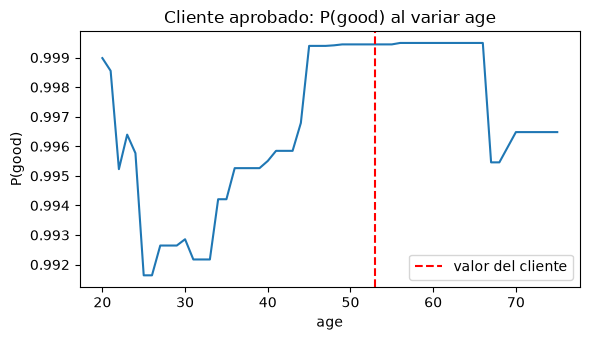
\includegraphics[width=0.6\textwidth]{figs/age_curva.png}
\caption{$P(\text{good})$ del cliente aprobado al variar solo \texttt{age}.}
\end{figure}

\begin{tcolorbox}[colback=yellow!12, colframe=orange!70!black, boxrule=0.5pt, left=4pt, right=4pt]
\textbf{Pregunta.} Identifique el cliente y la variable donde LIME y SHAP discrepan más. Proponga una hipótesis y pruébela con datos. ¿Se debe a localidad, no linealidad o interacción?
\end{tcolorbox}

La mayor discrepancia está en el cliente aprobado, en la variable \texttt{age}. Como LIME explica en probabilidad y SHAP en log-odds, se compararon las importancias normalizadas por la suma de cada método: \texttt{age} tiene 0.13 en LIME y 0.16 en SHAP. Es la brecha más grande de las 60 combinaciones, aunque es pequeña (\(\approx\) 3 puntos porcentuales).

La hipótesis es que se debe a la no linealidad de la sigmoide. Este cliente tiene \(p \approx 1\) (\(f \approx 7.5\)), así que en probabilidad el modelo está saturado: \texttt{age} casi no mueve \(P\)(good), aunque en log-odds sí tenga peso.

Se hicieron tres pruebas:

\begin{enumerate}
\def\labelenumi{\arabic{enumi}.}
\tightlist
\item
  \textbf{Variar \texttt{age}:} en probabilidad, la predicción solo va de 0.99 a \(\approx\) 1.00, con un pequeño escalón cerca de los 45 años. En log-odds, va de 4.8 a 7.6.
\item
  \textbf{Bajar \(\sigma_{rel}\) (más localidad):} la importancia de \texttt{age} en LIME solo sube de 0.13 a 0.14. La localidad no cierra la brecha.
\item
  \textbf{Usar LIME sobre el log-odds:} \texttt{age} sube a 0.14, el Spearman con SHAP pasa de 0.68 a 0.82 y el \(R^2_w\) de 0.26 a 0.39.
\end{enumerate}

La discrepancia se debe principalmente a la no linealidad, tanto por la saturación de la sigmoide como por el escalón en \texttt{age}, y no a la localidad. Como la brecha no se cierra del todo, el resto probablemente viene de interacciones que un modelo lineal no puede capturar.

\subsubsection*{(c) Elección de $K$}
\begin{figure}[H]
\centering
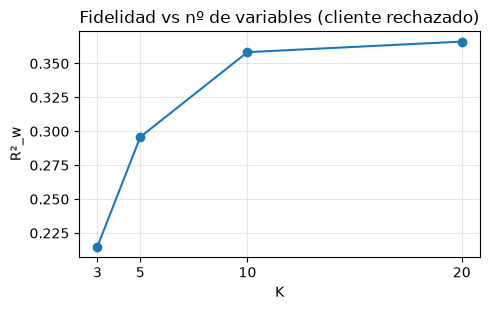
\includegraphics[width=0.5\textwidth]{figs/r2_vs_k.png}
\caption{Fidelidad $R^2_w$ según $K$ (cliente rechazado).}
\end{figure}

\begin{tcolorbox}[colback=yellow!12, colframe=orange!70!black, boxrule=0.5pt, left=4pt, right=4pt]
\textbf{Pregunta.} Con la tabla de \(R^2_w\) según \(K\), elija un \(K\) y justifique (fidelidad y comprensibilidad). ¿Qué fidelidad mínima aceptaría para una decisión de crédito? ¿Qué haría si no se alcanza?
\end{tcolorbox}

\begin{longtable}[]{@{}lcccc@{}}
\toprule\noalign{}
\(K\) & 3 & 5 & 10 & 20 \\
\midrule\noalign{}
\endhead
\bottomrule\noalign{}
\endlastfoot
\(R^2_w\) & 0.21 & 0.30 & 0.36 & 0.37 \\
\end{longtable}

Se eligió \(K = 5\). Con 5 variables se obtiene cerca del 80 \% de la fidelidad que da usar las 20 (\(0.30 / 0.37\)), y la curva casi no mejora después de \(K = 10\). Además, una explicación de 5 variables se puede leer y entender de un vistazo, mientras que una de 20 no.

Para justificar una decisión de crédito, se pediría al menos \(R^2_w \approx 0.8\)--\(0.9\). La explicación debe reproducir lo que hace el modelo, no solo aproximarlo a grandes rasgos. Aquí ningún \(K\) llega ni a 0.4.

Si no se alcanza esa fidelidad, no se usaría LIME para justificar la decisión, y se reportaría el \(R^2_w\) como limitación. En su lugar se usaría TreeSHAP, que suma exacto (se verificó un error de \(\sim10^{-7}\)), o un modelo local más flexible, como un árbol poco profundo que capture interacciones.

\subsubsection*{(d) Contrafactuales vs.\ variables de mayor $|\phi|$}
\begin{tcolorbox}[colback=yellow!12, colframe=orange!70!black, boxrule=0.5pt, left=4pt, right=4pt]
\textbf{Pregunta.} Compare las variables de los contrafactuales con las tres de mayor \(|\phi|\). Identifique una de \(|\phi|\) alto que no aparece y explique con números por qué. ¿Qué pregunta responde SHAP y cuál el contrafactual?
\end{tcolorbox}

Las tres variables con mayor \(|\phi|\) en el cliente rechazado son \texttt{credit\_history} (\(-1.26\)), \texttt{savings\_status} (\(+1.03\)) y \texttt{credit\_amount} (\(-0.99\)). Los contrafactuales cambian \texttt{checking\_status}, \texttt{credit\_amount}, \texttt{duration} e \texttt{installment\_commitment}. Solo \texttt{credit\_amount} aparece en ambas listas.

\texttt{credit\_history} tiene el \(|\phi|\) más alto (\(-1.26\) log-odds, unos \(-0.27\) en probabilidad) y es la variable que más empuja hacia el rechazo, pero no aparece en ningún contrafactual. La razón es que no es accionable: describe el pasado del cliente y no se puede cambiar de forma realista. La búsqueda solo modifica las 5 variables accionables, así que en los 20\,000 candidatos conserva su valor (\texttt{all paid}) y su \(-1.26\) queda intacto en todos los contrafactuales.

\texttt{savings\_status} tampoco aparece, pero por otra razón. Su contribución es positiva (\(+1.03\)) y el cliente ya está en la categoría con mayor tasa de \emph{good} en train (\(\geq\) 1000, 0.89). Se verificó cambiando solo \texttt{savings\_status} y dejando el resto fijo: con \(\geq\) 1000 la probabilidad es 0.052, con \emph{no known savings} (0.82 de \emph{good} en train) baja a 0.048, y con las otras tres categorías queda en \(\approx\) 0.01. Aplicado sobre CF1 pasa lo mismo (0.745 con \(\geq\) 1000 y 0.731 con \emph{no known savings}). Es decir, ningún otro valor mejora la probabilidad, y el modelo no tiene nada que ganar al cambiarla.

En cambio, \texttt{checking\_status} aparece en dos contrafactuales (CF1 y CF2, con \(P = 0.75\) y \(0.55\)) sin estar en el top-3 (\(\phi = -0.58\)). Es una variable barata de cambiar, porque cuesta solo 1 punto de distancia. Es decir, una variable con \(|\phi|\) alto no es necesariamente una buena palanca, y una buena palanca no necesita tener \(|\phi|\) alto.

Las dos herramientas responden preguntas distintas. SHAP responde \emph{¿por qué el modelo dio esta probabilidad?}, midiendo cuánto aportó cada variable respecto al cliente promedio. El contrafactual responde \emph{¿qué es lo mínimo y realizable que tendría que cambiar para que la decisión fuera otra?}

\newpage
\section*{Task 4 --- Validación de Grad-CAM}

\textit{El código de todo el Task 4 (4.1, 4.2 y el apoyo de 4.3) fue generado con IA (detallado en \texttt{AI.md}); las respuestas son mías.}

\subsection*{Task 4.1 --- Deletion e insertion}
\textbf{Instrucciones.}
\begin{itemize}
  \item Validar el mapa de Grad-CAM del Task 1.2 en las tres imágenes (clase top-1) con $P=20$ pasos y 10 órdenes aleatorios.
  \item Deletion: ordenar los píxeles de $224\times224$ por el valor del mapa de mayor a menor y reemplazar por gris la fracción $k/P$ más importante; $\mathrm{AUC}_{del}=\frac1P\sum_kc_k$.
  \item Insertion: partir de una versión desenfocada (gaussiano, $\sigma=10$ px) e insertar progresivamente los píxeles originales más importantes; $\mathrm{AUC}_{ins}$ igual. Repetir con 10 órdenes aleatorios (media y desviación estándar) y presentar una tabla por imagen con la diferencia respecto al azar \cite{petsiuk2018}.
\end{itemize}

\begin{figure}[H]
\centering
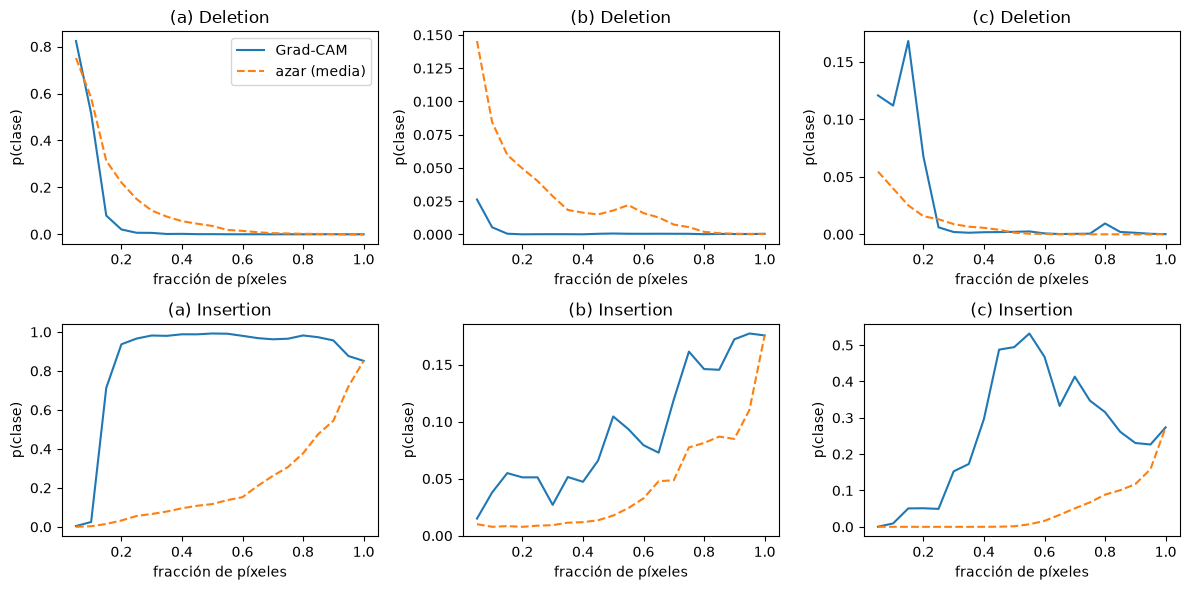
\includegraphics[width=\linewidth]{figs/del_ins.png}
\caption{Curvas de deletion (arriba) e insertion (abajo): Grad-CAM frente al promedio de los órdenes aleatorios.}
\end{figure}

\begin{table}[H]
\centering
\small
\begin{tabular}{llrrr}
\toprule
Imagen & Métrica & Grad-CAM & Azar ($\mu\pm\sigma$) & $z$ \\
\midrule
(a) espresso & AUC deletion & 0.073 & $0.119\pm0.009$ & $-5.4$ \\
 & AUC insertion & 0.854 & $0.231\pm0.021$ & $+30.0$ \\
(b) cup & AUC deletion & 0.002 & $0.027\pm0.007$ & $-3.7$ \\
 & AUC insertion & 0.092 & $0.044\pm0.008$ & $+6.3$ \\
(c) bell cote & AUC deletion & 0.025 & $0.009\pm0.003$ & $+5.6$ \\
 & AUC insertion & 0.258 & $0.046\pm0.009$ & $+24.3$ \\
\bottomrule
\end{tabular}
\caption{Deletion (menor es mejor) e insertion (mayor es mejor): Grad-CAM frente a 10 órdenes aleatorios; $z=(\text{AUC}_{mapa}-\mu)/\sigma$.}
\end{table}

\subsection*{Task 4.2 --- Aleatorización de parámetros en cascada}
\textbf{Instrucciones.}
\begin{itemize}
  \item Reinicializar con la inicialización por defecto de PyTorch, de forma acumulativa, \texttt{fc}, luego \texttt{layer4}, \texttt{layer3}, \texttt{layer2}, \texttt{layer1} y \texttt{conv1} \cite{adebayo2018}.
  \item En cada etapa calcular el mapa de Grad-CAM de $7\times7$ para la clase top-1 del modelo original y su correlación de Spearman con el mapa original; presentar una tabla (3 imágenes $\times$ 6 etapas).
\end{itemize}

\begin{table}[H]
\centering
\small
\begin{tabular}{lrrrrrr}
\toprule
Imagen & + fc & + layer4 & + layer3 & + layer2 & + layer1 & + conv1 \\
\midrule
(a) & $-0.007$ & 0.179 & $-0.002$ & $-0.236$ & 0.074 & $-0.037$ \\
(b) & 0.282 & 0.348 & 0.165 & 0.381 & 0.198 & $-0.093$ \\
(c) & $-0.431$ & 0.305 & 0.052 & 0.167 & 0.294 & 0.184 \\
\bottomrule
\end{tabular}
\caption{Correlación de Spearman con el mapa original de $7\times7$ en cada etapa acumulativa de la cascada.}
\end{table}

\subsection*{Task 4.3 --- Preguntas}
\subsubsection*{(a) Grad-CAM vs.\ azar, forma de las curvas y referencia desenfocada}
\begin{tcolorbox}[colback=yellow!12, colframe=orange!70!black, boxrule=0.5pt, left=4pt, right=4pt]
\textbf{Pregunta.} ¿Grad-CAM supera al azar en deletion e insertion y por cuántas desviaciones estándar? Explique la forma de las curvas (mapa \(7\times7\)). Repita deletion en la imagen (a) con referencia desenfocada en vez de gris y compare los AUC.
\end{tcolorbox}

En insertion, Grad-CAM supera al azar en las tres imágenes, por \(+30\sigma\) (a), \(+6\sigma\) (b) y \(+24\sigma\) (c). En deletion, menor es mejor: el AUC queda por debajo del azar en (a) por \(5\sigma\) y en (b) por \(4\sigma\). En (c) parece peor que el azar (\(+6\sigma\)), pero esto es un artefacto de la comparación, como se explica abajo.

Las curvas son abruptas, casi escalonadas. Como el mapa tiene solo \(7\times7 = 49\) celdas, cada paso de 5 \% de píxeles equivale a \(\approx\) 2.5 celdas. En (a), quitar el 20 \% de píxeles más importantes ya baja la probabilidad a \(\approx\) 0, e insertarlos la sube a \(\approx\) 0.94. El mapa ordena bloques grandes, no píxeles individuales.

En (c), el mapa señala el fondo (ver 1.4(c)). El azar por píxeles sueltos genera ruido que el modelo nunca vio, y eso hunde la probabilidad de cualquier clase (AUC \(\approx\) 0.007). Si el azar se hace por bloques de \(32\times32\), que es una comparación más justa, su AUC es \(\approx\) \(0.07 \pm 0.03\). Grad-CAM (\(\approx\) 0.025) queda por debajo, es decir, mejor que el azar, aunque sin una diferencia clara (\(\approx -1.3\sigma\)).

Con referencia desenfocada en la imagen (a), el AUC de deletion sube de \(\approx\) 0.07 (gris) a \(\approx\) 0.22. El azar con desenfoque da \(\approx\) \(0.18 \pm 0.03\), así que \(z \approx +1.4\): con desenfoque, Grad-CAM ya no supera al azar. Deletion depende mucho de la referencia: los parches grises son ruido que derrumba la probabilidad con facilidad, mientras que el desenfoque conserva el color y las formas generales.

\subsubsection*{(b) Cascada y predicción para \texttt{fc} aleatorizado}
\begin{tcolorbox}[colback=yellow!12, colframe=orange!70!black, boxrule=0.5pt, left=4pt, right=4pt]
\textbf{Pregunta.} ¿En qué etapa de la cascada cae el Spearman por debajo de 0.3 en cada imagen? Dado que \(\alpha_k^c=w_k^c/Z\), prediga qué pasa con el mapa cuando solo se aleatoriza \texttt{fc} y compare con la primera etapa.
\end{tcolorbox}

En las tres imágenes, el Spearman cae por debajo de 0.3 desde la primera etapa (\texttt{fc}): \(-0.01\) en (a), \(0.28\) en (b) y \(-0.43\) en (c).

Esto es lo que se esperaba. Como \(\alpha_k^c = w_k^c/Z\), si \texttt{fc} tiene pesos aleatorios \(w'\), el mapa pasa a ser \(\mathrm{ReLU}\big(\sum_k w'_k A^k / Z\big)\), es decir, una combinación aleatoria de canales, así que el Spearman debería ser \(\approx\) 0. Esto se verificó numéricamente: \(\max|\alpha - w'/Z| \sim 10^{-10}\).

El ruido de \(\pm\)0.14 es la dispersión de la correlación entre dos mapas sin relación con 49 celdas (\(1/\sqrt{48}\)). Con eso, (a) coincide con la predicción y (b) queda cerca (2 desviaciones). En cambio, (c) con \(-0.43\) está a \(\approx\) 3 desviaciones de 0, o sea que no es \(\approx\) 0: el mapa aleatorio ilumina justo lo que el original apagaba (con una sola semilla no se sabe si es real). Además, la cascada no es monótona: (b) vuelve a superar 0.3 en \texttt{layer4} (0.35) y \texttt{layer2} (0.38).

El método pasa el sanity check, porque el mapa depende de los pesos aprendidos. Pero en este ResNet toda la información de clase pasa por \texttt{fc}, así que la prueba no permite saber si las capas convolucionales aportan algo por su cuenta.

\subsubsection*{(c) Audiencias y riesgo de contrafactuales}
\begin{tcolorbox}[colback=yellow!12, colframe=orange!70!black, boxrule=0.5pt, left=4pt, right=4pt]
\textbf{Pregunta.} Para el modelo de crédito, indique qué explicación entregaría a (i) la persona solicitante, (ii) un oficial de cumplimiento y (iii) un regulador, con qué validaciones respaldadas por sus números y qué no entregaría. ¿Por qué un contrafactual como el de 3.4 sería un riesgo en un sistema de detección de lavado (Proyecto 2) y qué entregaría en su lugar?
\end{tcolorbox}

Como contexto, el modelo es modesto: exactitud \(\approx\) 0.78 y AUC \(\approx\) 0.77, así que ninguna explicación debería presentarse como más precisa de lo que es.

\textbf{Solicitante.} Se le daría una explicación corta en palabras con las 2--3 razones principales según TreeSHAP, por ejemplo que el monto del crédito y el historial pesaron en contra. Esto se respalda con que SHAP suma exacto (error \(\sim10^{-7}\)). No se le daría un valor \(\phi\) en log-odds, que no significa nada para esa persona, ni la explicación de LIME (\(R^2_w \approx 0.3\)), que reproduce poco del modelo. Tampoco se le diría que \texttt{credit\_history} es algo que pueda cambiar. Un contrafactual solo se le daría si es realista y estable, y CF1 no lo es: pide cerrar la cuenta corriente y pedir 7 unidades menos, y ese cambio de monto solo funciona porque cae en un corte de los árboles. CF2 no sirve de alternativa, porque es estrictamente peor (los mismos cambios más \texttt{duration}, con \(P = 0.55\) frente a 0.75).

\textbf{Oficial de cumplimiento.} Necesita revisar el modelo caso por caso, así que se le daría la cascada de cada cliente, el beeswarm global y la comparación entre SHAP y permutación. Lo respaldan que SHAP suma exacto, que el Shapley calculado a mano coincide con \texttt{shap} (\(\sim10^{-8}\)) y que el Spearman entre SHAP y permutación es \(\approx\) 0.70. No se le daría LIME como justificación principal, y tampoco importancias de variables duplicadas sin advertirlo, porque el crédito se reparte entre las copias y cada una parece valer \(\approx\) 0.30 en vez de \(\approx\) 0.49.

\textbf{Regulador.} Se le daría la documentación completa: TreeSHAP global y local, los límites de los datos y una revisión de las variables protegidas (\texttt{age} aporta \(+1.09\) al cliente aprobado). A lo anterior se suman la estabilidad de LIME (Jaccard 1.0 con \(N \geq 2000\)) y los sanity checks. No se le presentarían los contrafactuales como prueba de causalidad ni explicaciones sin su fidelidad reportada.

\textbf{Riesgo en detección de lavado.} Un contrafactual como el de 3.4 le diría al sospechoso exactamente qué cambiar para no ser detectado, por ejemplo fraccionar montos por debajo de cierto umbral. Sería una guía para evadir el sistema, y además le revelaría que está siendo investigado. En su lugar, a los analistas internos se les darían atribuciones tipo SHAP que muestren qué señales generaron la alerta, con acceso restringido. Al cliente se le daría solo un aviso genérico, sin umbrales ni variables, y al regulador una validación global del modelo, con explicaciones agregadas y sanity checks.

\newpage

\printbibliography

\end{document}
